% Desenvolvido para o IFSP por: Prof. Dr. David Buzatto (Versão 1.0.2, Data: 31/01/2023)
% Acessado em <https://github.com/davidbuzatto/TemplatesTrabalhosIFSPSBV/tree/master/Template%20Latex%20-%20Apresentacao%20-%20IFSP%20-%20SBV> em 02/02/2023
% Licença Creative Commons CC BY 4.0
% Adaptado para a UFMG por: Dra. Cecilia F. Fiorini (Data: 02/02/2023)
% Adaptado para o Macro em 10/10/2024

\documentclass[10pt,aspectratio=169]{beamer}
\usepackage[utf8]{inputenc}

% a opção hideSubsectionTitle esconde o título das subseções
\usepackage[hideSubsectionTitle]{estruturaApresentacao}
\usepackage[round]{natbib}
\bibliographystyle{abbrvnat}
% \usepackage[alf,abnt-emphasize=bf]{abntex2cite}
\usepackage{verbatim}
% \usepackage{microtype}
\usepackage{lmodern}
\usepackage{amsmath,amsfonts,amssymb} 
% \usepackage{newtxmath}
\usepackage{siunitx}
\usepackage{import}
\usepackage[labelformat=empty]{caption}
\usepackage{subfig}
\usepackage{xcolor}
\usepackage{transparent}
\usepackage{tikz}


\usetikzlibrary{shapes.geometric, arrows}
\tikzstyle{block} = [rectangle, rounded corners, minimum width=3.5cm, minimum height=1cm, text centered, draw=black, fill=UFMGExemplos!10, text width=4cm]
\tikzstyle{arrow} = [thick,->,>=stealth]


% \usepackage{newtxmath}

\sisetup{exponent-product=\cdot}
\DeclareMathOperator{\Lop}{L}
\DeclareRobustCommand{\SL}[1][]{%
  \!\;\mathcal{S}%
  \if\relax\detokenize{#1}\relax%
  \else%
    \!\left(#1\right)%
  \fi%
}


\begin{document}

\titulo{Constructive Vector Fields for Path Following in Matrix Lie Groups}
% caso não haja, comente a linha abaixo
% \subtitulo{subtítulo (se houver)}
\nome{}
\autor{Felipe Bartelt de Assis Pessoa}
\orientador{Luciano Cunha de Araújo Pimenta}
% caso não haja, comente a linha abaixo
\coorientador{Vinicius Mariano Gonçalves}

% \curso{Nome do Curso}

% exemplos
%\curso{Bacharelado em Ciência da Computação}
% \curso{Mestrado em Engenharia Elétrica}
%\curso{Especialização em Desenvolvimento de Aplicações para Dispositivos Móveis}

\local{Belo Horizonte}
\dia{21}
\mes{Fevereiro}
\ano{2025}


% !TeX root = Template Latex - Apresentacao - IFSP - SBV.tex
% não mexa!

\begin{frame}[plain]
    
    \begin{tikzpicture}[overlay,remember picture]
        \node[left=-0.15cm] at (current page.0){
            
\includegraphics[scale=0.202]{../figures/capa}
        };
        % comente a linha abaixo, caso não haja uma logo de conferencia
        % \node[anchor=north west, xshift=0.3cm, yshift=-0.1cm] at (current page.north west) {
        %     \includegraphics[scale=0.3]{imagens/Logocbasba.png}  % Ajuste a escala conforme necessário
        % };
    \end{tikzpicture}
    
    \titlepage
    
\end{frame}

% \section[Agenda]{}

% \begin{frame}
%     \frametitle{Agenda}
%     \tableofcontents
% \end{frame}
% !TeX root = Template Latex - Apresentacao - IFSP - SBV.tex

\section{Introduction}
\begin{frame}{Motivation}
    \begin{columns}[c]
    
        \begin{column}{0.6\linewidth}
            \begin{itemize}
                \item Generalize the vector field strategy in \citet{Rezende2022} to allow more motion possibilities, including rotations;
                \item Gain deeper insight into vector field properties through generalization;
                \item Facilitate path following for systems with both translational and rotational motion, such as omnidirectional UAVs and robotic manipulators.
            \end{itemize}
        \end{column}

        \begin{column}{0.4\linewidth}
 
            \begin{figure}
                \centering
                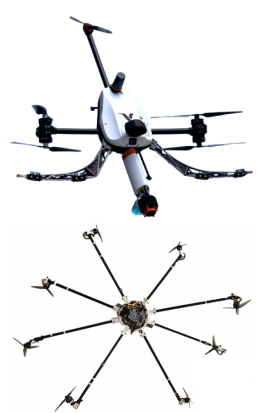
\includegraphics[width=.8\linewidth]{../figures/voliro_omni_vertical.png}
            \end{figure}

        \end{column}

    \end{columns}
    
\end{frame}

\begin{frame}{Contributions}
    \begin{itemize}
        \item Development of a novel vector field guidance strategy applicable to systems with an inherent matrix Lie group structure;
        \item Implementation framework for $\text{SE}(3)$ systems, providing all necessary tools for practical application of the proposed strategy;
        \item Validation through kinematic simulations in $\text{SE}(3)$ and $\text{SO}^+(3,1)$, demonstrating the theoretical results and their practical implications;
        \item Design of an adaptive control strategy for collaborative simulations in $\mathbb{R}^3 \times \text{SO}(3)$, where the vector field guidance strategy generates reference velocities for dynamic control.
    \end{itemize}
\end{frame}

\begin{frame}{Background}
    \begin{tikzpicture}
        % Nodes
        \node (coursework) [block] {Coursework \& assignments};
        \node (culbertson) [block, right of=coursework, xshift=4cm] {Adapt \citet{Culbertson2021} to  vector field of \citet{Rezende2022}};
        % \node (rezende) [block, right of=culbertson, xshift=4cm] {Adaptation to \\ \citet{Rezende2022}};
        \node (pessoa) [block, right of=culbertson, xshift=4cm] {Include orientation \\ $\mathbb{R}^3 \times \text{SO}(3)$  \citep{Pessoa2024}};
        % \node (pessoa) [block, below of=rezende, yshift=-2cm] {Extension to \\ $\mathbb{R}^3 \times \text{SO}(3)$ \\ \citet{Pessoa2024}};
        \node (generalization) [block, below of=pessoa, yshift=-2cm] {Insights into\\ deeper properties};
        % \node (generalization) [block, left of=pessoa, xshift=-4cm] {Generalization to \\ Matrix Lie Groups};
        \node (automatica) [block, left of=generalization, xshift=-4cm] {Generalization to Matrix Lie Groups\\ (\textit{Automatica} submission)};
    
        % Arrows
        \draw [arrow] (coursework) -- (culbertson);
        \draw [arrow] (culbertson) -- (pessoa);
        % \draw [arrow] (rezende) -- (pessoa);
        \draw [arrow] (pessoa) -- (generalization);
        \draw [arrow] (generalization) -- (automatica);
    \end{tikzpicture}
\end{frame}

% \begin{frame}

%     \frametitle{Motivação}
%      Incorporar orientação ao campo de \citet{Rezende2022}, adotando o modelo:
%      \begin{align*}
%          \boldsymbol{\xi} = \begin{bmatrix}
%              \dot{\mathbf{p}} \\ \boldsymbol{\omega}
%          \end{bmatrix} = \begin{bmatrix}
%              \dot{\mathbf{p}}_d \\ \boldsymbol{\omega}_d \end{bmatrix}.
%      \end{align*}

%      Exemplos de aplicação:
%     \begin{itemize}
%        	\item Controle de um VANT omnidirecional para circular uma curva com orientações predefinidas.
%         \item Manipulação de um objeto grande, que deve seguir uma sequência específica de posições e orientações durante o transporte.
%     \end{itemize}
%     % \vspace{0.5cm}
% \end{frame}
% % !TeX root = Template Latex - Apresentacao - IFSP - SBV.tex

\section{Theoretical Background}

\begin{frame}
    \frametitle{Vector field in Euclidean space}
    \begin{columns}[c]
        \begin{column}{7cm}
            The vector field strategy in \citet{Rezende2022} uses a parametric representation of the curve and is characterized by:
            \begin{itemize}
                \item A distance function $D$;
                \item $\dot{D}=(\nabla D)^\top\boldsymbol{\xi}=-\boldsymbol{\xi}_N^\top\boldsymbol{\xi}$;
                \item the tangent component is depends on the curve only;
                \item orthogonality between normal and tangent components;
                \item vector field $\Psi(\mathbf{h})=k_N(D)\boldsymbol{\xi}_N(\mathbf{h}) + k_T(D)\boldsymbol{\xi}_T(\mathbf{h})$.
            \end{itemize}
            
        \end{column}
        \begin{column}{8cm}
           \begin{figure}[ht!]
            \centering
            \def\svgwidth{\linewidth}
            {\footnotesize\import{imagens/}{plotly_vf2.pdf_tex}}
        \end{figure}
        \end{column}
    \end{columns}
\end{frame}
% !TeX root = Template Latex - Apresentacao - IFSP - SBV.tex
\section{Theoretical Background}

\begin{frame}
    \frametitle{Vector field in Euclidean space}
    \begin{columns}[c]
        \begin{column}{7cm}
            The vector field strategy in \citet{Rezende2022} is based on a parametric curve representation and is characterized by:
            \begin{itemize}
                \item A distance function $D$;
                \item $\dot{D}=\nabla D\boldsymbol{\xi}=-\boldsymbol{\xi}_N^\top\boldsymbol{\xi}$;
                \item Tangent component depends only on the curve;
                \item Normal and tangent components are orthogonal;
                \item Absence of local minima outside the curve;
                \item Vector field $\Psi(\mathbf{h})=k_N(D)\boldsymbol{\xi}_N(\mathbf{h}) + k_T(D)\boldsymbol{\xi}_T(\mathbf{h})$.
            \end{itemize}
            
        \end{column}
        \begin{column}{8cm}
           \begin{figure}[ht!]
            \centering
            \def\svgwidth{\linewidth}
            {\footnotesize\import{../figures/}{plotly_vf2.pdf_tex}}
        \end{figure}
        \end{column}
    \end{columns}
\end{frame}
\begin{frame}{Lie Groups and Lie algebras}
    \begin{columns}[c]
        \begin{column}{0.5\linewidth}
            \begin{exampleblock}{Lie group $G$}
                Manifolds with group structure. The group operation and inverse map are continuous and smooth.
                \linebreak

                E.g.: set of rotation matrices $\text{SO}(3)$.
            \end{exampleblock}
            \begin{exampleblock}{Lie algebra $\mathfrak{g}$}
                Tangent space of $G$ at the identity.
                \linebreak

                E.g.: skew-symmetric matrices for $\text{SO}(3)$.
            \end{exampleblock}
        \end{column}
        \begin{column}{0.5\linewidth}
            \begin{exampleblock}{Exponential map}
                Maps elements of $\mathfrak{g}$ to $G$. For matrix Lie groups: $\exp(\mathbf{A})=\sum_{i=0}^\infty \frac{\mathbf{A}^n}{n!} = \mathbf{X} \in G$.

                Not always surjective.
            \end{exampleblock}
            \begin{exampleblock}{$\mathcal{S}$ map}
                Linear map from $\mathbb{R}^m$ to $\mathfrak{g}$, relating velocities to tangent space elements.
                \linebreak

                E.g.: angular velocities $\to$ skew-symmetric matrices in $\mathfrak{so}(3)$.
            \end{exampleblock}    
        \end{column}
    \end{columns}
\end{frame}

% !TeX root = Template Latex - Apresentacao - IFSP - SBV.tex
\section{Vector Field}
% \subsection{Controller Design}
\begin{frame}{Formulation}
    \begin{figure}[ht]
        \centering
        \begin{tikzpicture}[
                block/.style={draw, rectangle, minimum height=1.2cm, minimum width=2.4cm, align=center},
                arrow/.style={->, >=stealth, thick},
                label/.style={font=\small}
            ]
            
            % Nodes
            \node[block] (controller) {Vector Field};
            \node[block, right=2cm of controller] (plant) {System};
            % \node[block, below=1cm of plant] (estimation) {Estimation of $\theta_c$};
            
            % Arrows between blocks
            \draw[arrow] (controller) -- node[above, label] {$\Psi(\mathbf{H})$} (plant);
            % Input and Output Arrows
            \node[left=1.5cm of controller, yshift=0.25cm] (input) {Curve $\mathcal{C}\subset G$};
            \draw[arrow] (input) -- ($(controller.west)+(0,0.25)$);    
            \node[right=1.5cm of plant] (output) {$\mathbf{H}(t)\in G$};
            \draw[arrow] (plant.east) -- (output);    
            % Feedback loop
            % \draw[arrow] ($(plant.east)+(0.75,0)$) |- ++(0,-1.5) -| (aux) -| ($(controller.west)+(0,-0.25)$);
            \draw[arrow] 
            ($(plant.east)+(0.75,0)$) |- ++(0,-1.25)
            -|  ($(controller.west)+(-0.75,-0.25)$)                          
            -- ($(controller.west)+(0,-0.25)$);
        
        \end{tikzpicture}
    \end{figure}
    We assume the system model:
    \begin{align*}
        \dot{\mathbf{H}}(t)=\mathcal{S}\bigl(\boldsymbol{\xi}(t)\bigr)\mathbf{H}(t),\quad \mathbf{H}\in G,\  \boldsymbol{\xi}\in\mathbb{R}^m,
    \end{align*}

    The vector field is given by:
    \begin{align*} 
        \Psi\left(\mathbf{H}\right) \triangleq k_N(\mathbf{H})\boldsymbol{\xi}_N(\mathbf{H}) + k_T(\mathbf{H})\boldsymbol{\xi}_T(\mathbf{H}). 
    \end{align*}
    
\end{frame}

\begin{frame}{Gradient in Lie groups}
\begin{columns}[c]
        \begin{column}{0.6\linewidth}
            The $\Lop$ operator acts as a gradient while respecting Lie group constraints.
            \newline

            For any scalar function $f: G \to \mathbb{R}$, it is implicitly defined as:
            \begin{exampleblock}{L operator}
                {\centering $\displaystyle 
                \begin{aligned} \lim_{\varepsilon \rightarrow 0} \frac{1}{\varepsilon} \Biggl( f\Bigl(\exp\bigl(\SL[\boldsymbol{\zeta}]\varepsilon\bigr)\mathbf{G}\Bigr) - f\bigl(\mathbf{G}\bigr) \Biggr) &= \Lop[f](\mathbf{G}) \boldsymbol{\zeta} \ \forall\, \boldsymbol{\zeta} \in \mathbb{R}^m
                \\\left.\frac{d}{d\varepsilon}\biggl(f\Bigl(\exp\bigl(\SL[\boldsymbol{\zeta}]\varepsilon\bigr)\mathbf{G}\Bigr)\biggr)\right|_{\varepsilon=0} &= \Lop[f](\mathbf{G})\boldsymbol{\zeta}\ \forall\, \boldsymbol{\zeta} \in \mathbb{R}^m
                \end{aligned}$ 
                \par}%
            \end{exampleblock}
        \end{column}
        \begin{column}{0.4\linewidth}
           \begin{figure}[ht!]
                \centering
                \def\svgwidth{\linewidth}
                {\footnotesize\import{../figures/}{tangents.pdf_tex}}
            \end{figure}
        \end{column}
    \end{columns}
    
\end{frame}

\begin{frame}{Distances}
    The vector field formulation requires two distance functions:
    \begin{exampleblock}{EE-distance $\widehat{D}$}
        Measures the distance between two Lie group elements.

        \quad\emph{Positive definite:} $\widehat{D}(\mathbf{V}, \mathbf{W})\ge0,\ \widehat{D}(\mathbf{V},\mathbf{W})=0\iff\mathbf{V}=\mathbf{W};$

        \quad\emph{Differentiability:} at least once differentiable in both arguments almost everywhere.        
    \end{exampleblock}
    E.g.: for exponential Lie groups, an EE-distance is given by
    \begin{align*}
        \widehat{D}(\mathbf{V}, \mathbf{W}) = \bigl\|\log(\mathbf{V}^{-1}\mathbf{W})\bigr\|_F.
    \end{align*}

    \begin{exampleblock}{EC-distance $D$}
        Measures the distance between a Lie group element and a curve:

        {\centering $\displaystyle 
        \begin{aligned} D(\mathbf{H}) \triangleq \min_{\mathbf{Y}\in\mathcal{C}}\widehat{D}(\mathbf{H}, \mathbf{Y}) =
        \min_{s\in[0,1]} \widehat{D}\bigl(\mathbf{H}, \mathbf{H}_d(s)\bigr).
        \end{aligned}$ 
        \par}%
    \end{exampleblock}
\end{frame}

\begin{frame}{Components and Properties}
    \begin{columns}[c]
        \begin{column}{0.5\linewidth}
            Normal and tangent components:
            \begin{align*}
                \boldsymbol{\xi}_N(\mathbf{H}) &\triangleq -\Lop_{\mathbf{V}}[\widehat{D}]\Bigl(\mathbf{H}, \mathbf{H}_d(s^*)\Bigr)^{\top}\\
                \boldsymbol{\xi}_T(\mathbf{H}) &\triangleq  \SL^{-1}\biggl(\frac{d\mathbf{H}_d}{ds}(s^*)\mathbf{H}_d(s^*)^{-1}\biggr)
            \end{align*}

            Components are orthogonal if
                \begin{exampleblock}{Left-invariant distance}
                    {\centering $\displaystyle 
                    \begin{aligned} \widehat{D}(\mathbf{X}\mathbf{V}, \mathbf{X}\mathbf{W}) = \widehat{D}(\mathbf{V}, \mathbf{W})\,\forall\,\mathbf{V}, \mathbf{W}, \mathbf{X} \in G.
                    \end{aligned}$ 
                    \par}%
                \end{exampleblock}
                Absence of local minima outside the curve if
                \begin{exampleblock}{Chainable distance}
                    {\centering $\displaystyle
                    \begin{aligned}
                        \widehat{D}(\mathbf{V}, \mathbf{W}) = \widehat{D}\bigl(\mathbf{V}, \Phi_\sigma\bigr) + \widehat{D}\bigl(\Phi_\sigma, \mathbf{W} \bigr).
                    \end{aligned}$
                    \par}%
                \end{exampleblock}
        \end{column}
        \begin{column}{0.5\linewidth}
            \begin{figure}[ht!]
                \centering
                \def\svgwidth{\linewidth}
                {\scriptsize\import{../figures/}{invariant_chainable.pdf_tex}}
            \end{figure}
        \end{column}
    \end{columns}
    
\end{frame}

\begin{frame}{Sketch of proof}
    Let $\widehat{D}$ be a left-invariant and chainable EE-distance, then:
    \begin{align*}
        \dot{D} = \Lop_\mathbf{V}[\widehat{D}]\boldsymbol{\xi} + \bigl(\Lop_\mathbf{W}[\widehat{D}]\boldsymbol{\xi}_T\bigr)\frac{ds^*}{dt}.
    \end{align*}

    By the optimality condition of $D$, we have
    \begin{align*}
        \dot{D} = \Lop_\mathbf{V}[\widehat{D}]\boldsymbol{\xi} = -\boldsymbol{\xi}_N^\top\boldsymbol{\xi}.
    \end{align*}

    If the system follows the vector field, $\boldsymbol{\xi}=\Psi$, then
    \begin{align*}
        \dot{D} = -\boldsymbol{\xi}_N^\top(k_N\boldsymbol{\xi}_N + k_T\boldsymbol{\xi}_T)
         =-k_N\|\boldsymbol{\xi}_N\|^2 \le 0.
    \end{align*}

    Circulation relies on proper parametrization.
    
\end{frame}


% !TeX root = Template Latex - Apresentacao - IFSP - SBV.tex
\section{Results}
% \subsection{Simulations}
\begin{frame}{Kinematic control in $\text{SE}(3)$}
    The distance function has a simpler expression. Let
    \begin{align*}
        \mathbf{V}^{-1}\mathbf{W}
    = \begin{bmatrix}
        \mathbf{Q} & \mathbf{u} \\
        \mathbf{0} & 1
    \end{bmatrix},
    \end{align*}
    then
    \begin{align*}
        \widehat{D}(\mathbf{V},\mathbf{W}) = \|\log(\mathbf{V}^{-1}\mathbf{W})\|_F = \sqrt{2\theta^2 + \mathbf{u}^\top\bar{\mathbf{X}}\mathbf{u}},
    \end{align*}
    where
    \begin{align*}
        \theta &= \text{atan2}\left(\frac{1}{2\sqrt{2}}\|\mathbf{Q}{-}\mathbf{Q}^{\top}\|_F,\  \frac{1}{2}\bigl(\text{tr}(\mathbf{Q})-1\bigr)\right),\\
        \bar{\mathbf{X}} &= (1-2\beta_0)\mathbf{I} + \beta_0\bigl(\mathbf{Q} + \mathbf{Q}^\top\bigr),\\
        \beta_0&=\frac{2-2\cos\theta-\theta^2}{4(1 - \cos\theta)^2}.
    \end{align*}
\end{frame}

\begin{frame}{Kinematic control in $\text{SE}(3)$}
    Vector field gains:
    \begin{align*}
        k_N(\mathbf{H}) &= \tanh\bigl(20D(\mathbf{H})\bigr),\\
        k_T(\mathbf{H}) &= 1 - 0.5\tanh\bigl(D(\mathbf{H})\bigr).
    \end{align*}
    Lie algebra basis reflecting the mechanical twist:
    \begin{align*}
        \SL[\boldsymbol{\xi}] = \begin{bmatrix}
        0 & -\xi_6 & \xi_5 & \xi_1 \\
        \xi_6 & 0 & -\xi_4 & \xi_2 \\
        -\xi_5 & \xi_4 & 0 & \xi_3 \\
        0 & 0 & 0 & 0
        \end{bmatrix}.
    \end{align*}
    The normal and tangent components were numerically approximated. 
    
    The system was integrated using:
    \begin{align*}
        \mathbf{H}(t + \Delta t) \approx \exp\Bigl(\SL\bigl(\Psi(\mathbf{H})\bigr)\Delta t\Bigr)\mathbf{H}(t),
    \end{align*}
    with a time step of $\Delta t = \qty{1E-2}{\second}$. 
\end{frame}

\begin{frame}{Trajectory}
    \begin{figure}[ht!]
    \centering
    % First subfigure
    \subfloat{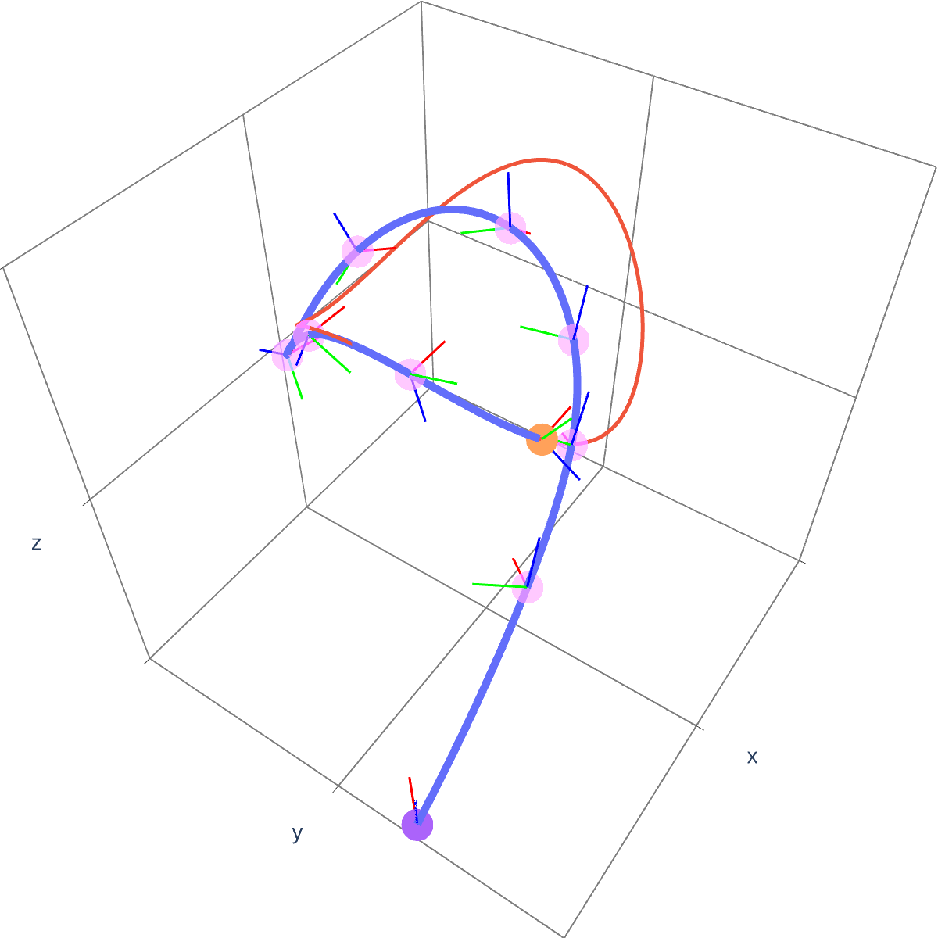
\includegraphics[width=0.32\textwidth]{../figures/vf_automatica_1.pdf}}\quad
    \subfloat{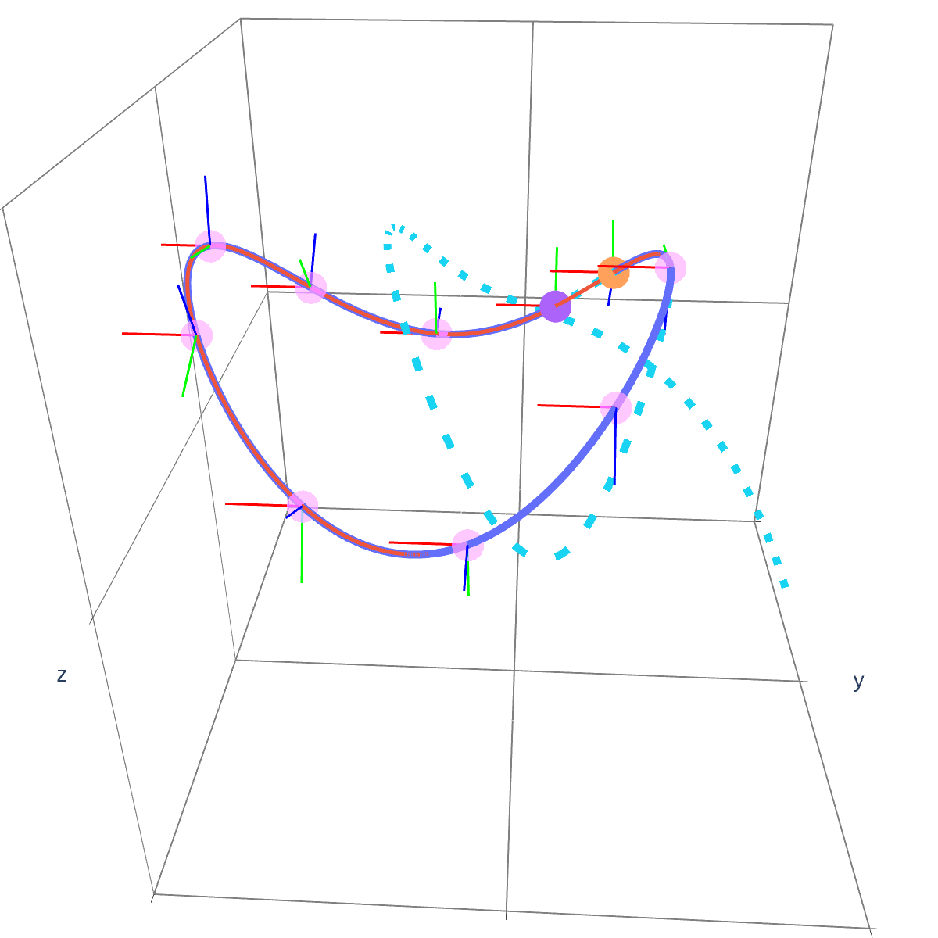
\includegraphics[width=0.32\textwidth]{../figures/vf_automatica_2.pdf}}
    \subfloat{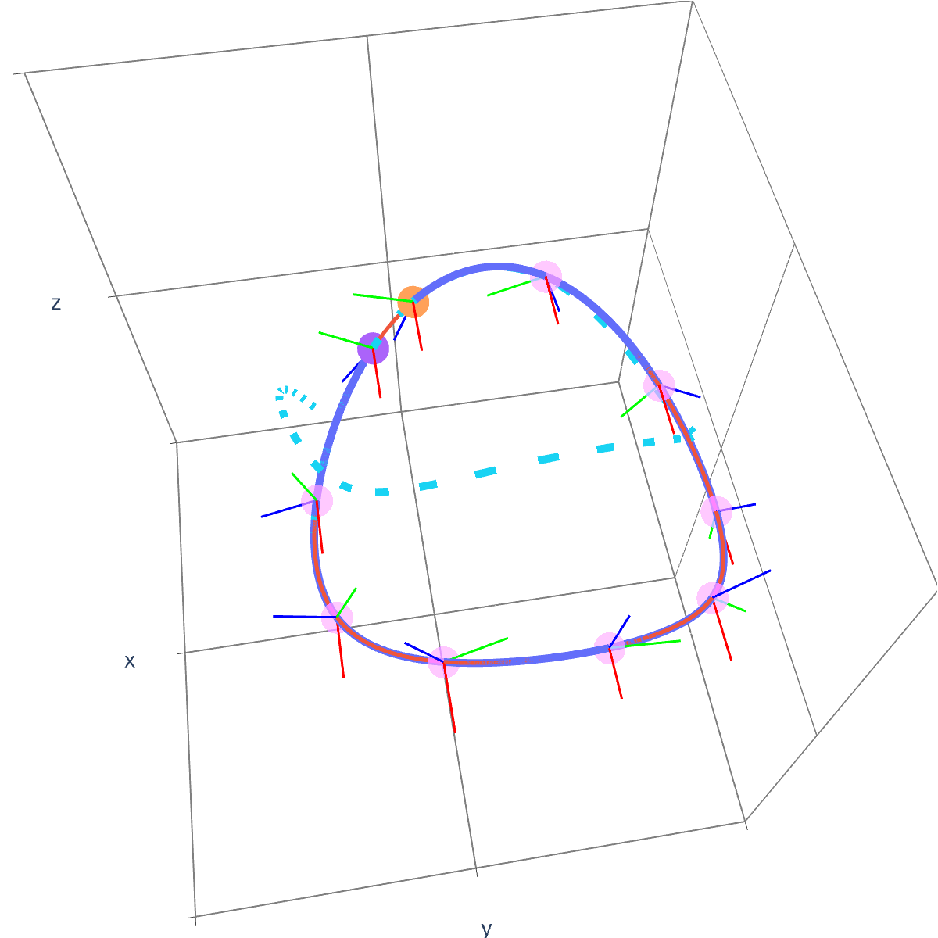
\includegraphics[width=0.32\textwidth]{../figures/vf_automatica_3.pdf}}
\end{figure}
\end{frame}

\begin{frame}{Distances}
    \begin{figure}[ht!]
        \centering
        \def\svgwidth{.9\linewidth}
        {\scriptsize\import{../figures/}{distance_pos_ori_D.pdf_tex}}
    \end{figure}
\end{frame}

\begin{frame}{Kinematic control in $\text{SO}^+(3,1)$}
    \begin{columns}[t]
        \begin{column}{0.5\linewidth}
            EE-distance:
            \begin{align*}
                \widehat{D}(\mathbf{V},\mathbf{W}) = \bigl\|\log(\mathbf{V}^{-1}\mathbf{W})\bigr\|_F
            \end{align*}
            Vector field gains:
            \begin{align*}
                k_N(\mathbf{H}) &= \tanh\bigl(\num{1000}D(\mathbf{H})\bigr)\\
                k_T(\mathbf{H}) &= 0.5\Bigl(1 - \tanh\bigl(100D(\mathbf{H})\bigr)\Bigr).
            \end{align*}
            Lie algebra isomorphism:
            \begin{align*}
                \SL[\boldsymbol{\xi}] = \begin{bmatrix}
                    0 & -\xi_3 & \xi_2 & \xi_4 \\
                    \xi_3 & 0 & -\xi_1 & \xi_5 \\
                    -\xi_2 & \xi_1 & 0 & \xi_6 \\
                    \xi_4 & \xi_5 & \xi_6 & 0
                \end{bmatrix}.
            \end{align*}
        \end{column}
        \begin{column}{0.5\linewidth}
            Parameterized curve:
            \begin{align*}
                \mathbf{H}_d(s) = \begin{bmatrix}
                    \gamma(s) & 0 & 0 & -\gamma(s) v(s)\\
                    0 & 1 & 0 & 0\\
                    0 & 0 & 1 & 0\\
                    -\gamma(s) v(s) & 0 & 0 & \gamma(s)
                \end{bmatrix},\label{eq:results-lorentz-curve-parametrization}
            \end{align*}
            where $v(s) = 0.9 + \frac{0.09}{2}(\cos(2\pi s) + 1)$, $\gamma(s) = \frac{1}{\sqrt{1 - v(s)^2}}$.
            
            Initial condition:
            \begin{align*}
                \mathbf{H}(0) = \exp\bigl(\SL[\boldsymbol{\xi}_0]\bigr),
            \end{align*}
            where $\boldsymbol{\xi}_0 = [0\ 0\ 0\ 0.7\ 0\ 0]^\top$.
        \end{column}

    \end{columns}
\end{frame}

\begin{frame}{Distance}
    \begin{figure}[ht!]
        \centering
        \def\svgwidth{.9\linewidth}
        {\scriptsize\import{../figures/}{lorentz_distanceD.pdf_tex}}
    \end{figure}
\end{frame}

\begin{frame}{Collaborative Manipulation}
    \begin{columns}[c]
        \begin{column}{0.4\linewidth}
            Each agent can measure the pose and velocity of the object's measurement point:

            \quad pose: $\boldsymbol{\chi} = (\mathbf{p}, \mathbf{R}) \in \mathbb{R}^3\times \text{SO}(3)$;
            
            \quad velocity: $\dot{\boldsymbol{\chi}} = \left[\dot{\mathbf{p}}^\top, \boldsymbol{\omega}^\top \right]^\top\in\mathbb{R}^6$;
            
            \quad acceleration: $\ddot{\boldsymbol{\chi}} = \left[\ddot{\mathbf{p}}^\top, \dot{\boldsymbol{\omega}}^\top \right]^\top\in\mathbb{R}^6$.

            System model:
            \begin{align*}
                \boldsymbol{\tau } = \mathbf {M}(\boldsymbol{\chi})\ddot{\boldsymbol{\chi}} + \mathbf {C}(\boldsymbol{\chi},\dot{\boldsymbol{\chi}})\dot{\boldsymbol{\chi}} + \mathbf{g},
            \end{align*}

            Reference model:
            \begin{align*}
                % \resizebox{0.91\columnwidth}{!}{%
                % $
                \alpha _i \left(\mathbf {M}(\boldsymbol{\chi})\dot{\Psi} + \mathbf {C}(\boldsymbol{\chi},\dot{\boldsymbol{\chi}})\Psi + \mathbf {g} \right) = \mathbf{Y}_o\mathbf{o}_i
                % $
                % }
            \end{align*}

            Unknowns: $m, \mathbb{I}_\text{cm}^\mathfrak{B}, \mathbf{r}_p, \mathbf{r}_i$
        \end{column}
        \begin{column}{0.6\linewidth}
            \begin{figure}[ht!]
                \centering
                \def\svgwidth{\linewidth}
                {\scriptsize\import{../figures/}{collaborative_scheme.pdf_tex}}
            \end{figure}
        \end{column}
    \end{columns}
\end{frame}

\begin{frame}{Vector Field}
    % \begin{columns}[t]
    %     \begin{column}{0.5\linewidth}
            Equivalent matrix Lie group: $\text{ISE}(3)$.

            Let
            \begin{align*}
                \mathbf{V}^{-1}\mathbf{W} = \begin{bmatrix}
                    \mathbf{Q} & \mathbf{0} & \mathbf{0}\\
                    \mathbf{0} & \mathbf{I} & \mathbf{u}\\
                    \mathbf{0} & \mathbf{0} & 1
                \end{bmatrix} \in \text{ISE}(3)\,,\,  \mathbf{Q}\in\text{SO}(3),\,\mathbf{u}\in\mathbb{R}^3,
            \end{align*}

            then the EE-distance is computed as:
            \begin{align*}
                \widehat{D}(\mathbf{V},\mathbf{W}) = \bigl\|\log(\mathbf{V}^{-1}\mathbf{W})\bigr\|_F = \sqrt{2\theta^2 + \|\mathbf{u}\|^2}.
            \end{align*}

            Isomorphism:
            \begin{align*}
                \SL[\boldsymbol{\xi}]= \begin{bmatrix}
                    \widehat{\mathcal{S}}(\boldsymbol{\omega}) & \mathbf{0} & \mathbf{0}\\
                    \mathbf{0} & \mathbf{0} & \mathbf{v}\\
                    \mathbf{0} & \mathbf{0} & 0
                \end{bmatrix},
            \end{align*}
            where $\boldsymbol{\xi} = [\mathbf{v}^\top\ \boldsymbol{\omega}^\top]^\top$.

           
    %     \end{column}
    %     \begin{column}{0.5\linewidth}
            
    %     \end{column}

    % \end{columns}
\end{frame}

\begin{frame}{Control}
    \begin{figure}[ht]
        \centering
        \resizebox{\textwidth}{!}{%
        \begin{tikzpicture}[
            block/.style={draw, rectangle, minimum height=1.2cm, minimum width=2.4cm, align=center},
            arrow/.style={->, >=stealth, thick},
            label/.style={font=\small},
            sumblock/.style={draw, circle, minimum size=0.8cm}
        ]
        
        % Nodes
        \node[block] (kinematic) {Vector Field};
        \node[block, right=2cm of kinematic] (refmodel) {Reference\\Model};
        % \node[block, right=2cm of kinematic] (plant) {Plant \\ $P(\theta)\to P_c(\theta_c)$};
        \node[block, right=1cm of refmodel] (control) {Dynamic\\Controller};
        \node[block, above=0.75cm of control] (estimation) {Estimation\\of $\mathbf{o}_i, \mathbf{r}_i$};
        \node[block, above=1cm of estimation, xshift=-1cm] (mapping) {Mapping\\$\mathbb{R}^3\times\text{SO}(3)\to\text{ISE}(3)$};
        \node[block, right=1cm of control] (plant) {System};
        \node[left=0.75cm of kinematic,yshift=-0.25cm] (input) {Curve $\mathcal{C}$};
        \node[sumblock, left=2cm of estimation, yshift=-0.25cm] (sum) {};
        \node at ([xshift=0.2cm]sum.west) {\(+\)};
        \node at ([yshift=-0.2cm]sum.north) {\(-\)};
        \node[right=1.5cm of plant] (output) {$\boldsymbol{\chi}$};
        
        % Arrows between blocks
        \draw[arrow] (input) -- ($(kinematic.west)+(0,-0.25cm)$);
        \draw[arrow] (plant.east) -- (output);
        % Ends in refmodel
        \draw[arrow] (kinematic) -- node[below, label] {$\Psi, \dot{\Psi}$} (refmodel);
        \draw[arrow] ($(plant.east)+(0.75, 0)$) |- ($(refmodel.south)+(0,-1)$) -| node[right, label,yshift=0.25cm] {$\boldsymbol{\chi}, \dot{\boldsymbol{\chi}}$} (refmodel.south);
        % Ends in System
        \draw[arrow] (control) -- node[above, label] {$\boldsymbol{\tau}_i$} (plant);
        % Ends in mapping
        \draw[arrow] ($(plant.east)+(0.75,0)$) |- (mapping.east) node[right, yshift=0.25cm, label] {$\boldsymbol{\chi}\in\mathbb{R}^3\times\text{SO}(3)$};
        % Ends in Estimation
        \draw[arrow] (sum.east) -- node[below,label] {$\boldsymbol{\zeta}$} ($(estimation.west)+(0,-0.25)$);
        \draw[arrow] ($(plant.east)+(0.75,0)$) |- (estimation.east) node[right, label, yshift=0.25cm] {$\boldsymbol{\chi}, \dot{\boldsymbol{\chi}}$};
        \draw[arrow] ($(refmodel.east)+(0.5,0)$) |- ($(estimation.west)+(0,0.25)$);
        % Ends in Vector Field
        \draw[arrow] (mapping.west) node[left, yshift=0.25cm, label] {$\mathbf{H}\in\text{ISE}(3)$} -| ($(kinematic.west)+(-0.75,1)$) |- ($(kinematic.west)+(0,0.25)$);
        % Ends in Control
        \draw[arrow] (estimation.south) -- node[right, label] {$\widehat{\mathbf{o}}_i, \widehat{\mathbf{r}}_i$} (control.north);
        \draw[arrow] (refmodel.east) -- node[below, label] {$\mathbf{Y}_o$} (control.west);
        \draw[arrow] ($(estimation.west)+(-0.25,-0.25)$) |- ($(control.west)+(0,0.25)$);
        \draw[arrow] ($(plant.east)+(0.75, 0)$) |- ($(control.south)+(0,-0.5)$) -| node[right, label,yshift=0.25cm] {$\boldsymbol{\chi}$} (control.south);
        % Ends in summation block
        \draw[arrow] ($(kinematic.east)+(1,0)$) |- node[left, label] {$\Psi$} (sum.west);
        \draw[arrow] ($(plant.east)+(0.75,0)$) |- ($(sum.north)+(0,1)$) -| node[left, label] {$\dot{\boldsymbol{\chi}}$} (sum.north);
        \end{tikzpicture}%
        }
    \end{figure}
\end{frame}

\begin{frame}{Trajectory}
    \begin{figure}[ht!]
        \centering
        % First subfigure
        \subfloat{\label{aa}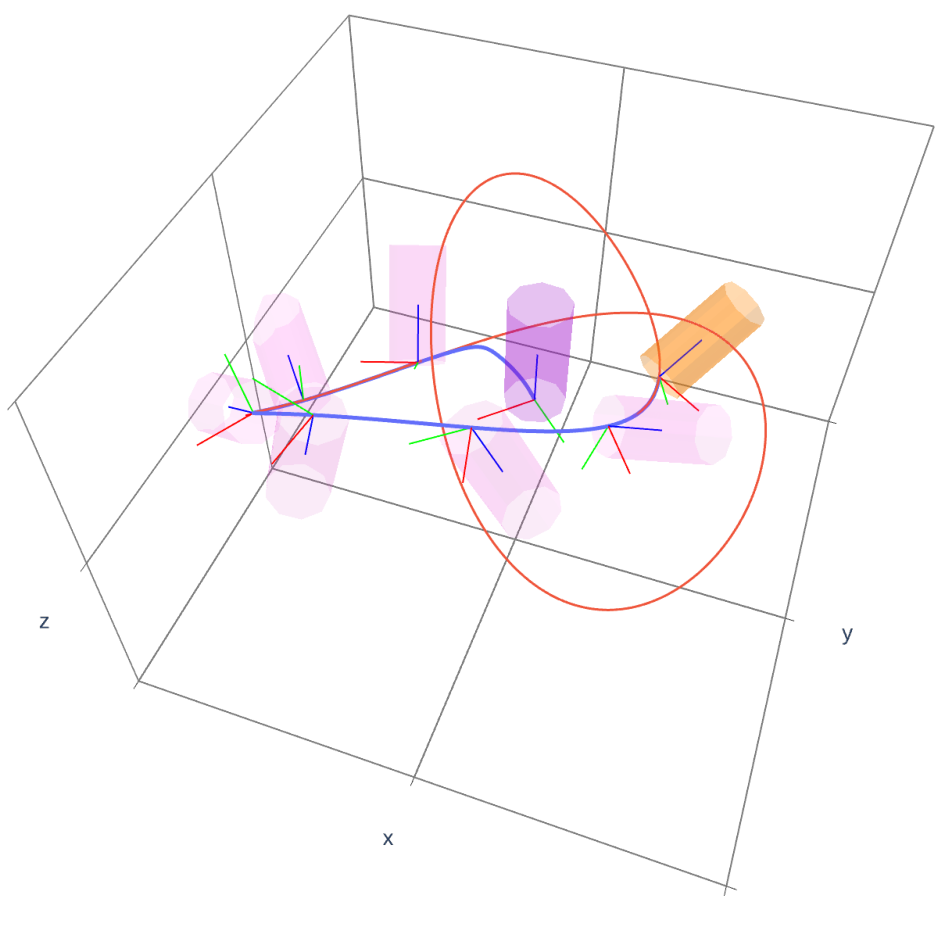
\includegraphics[width=0.32\textwidth]{../figures/adaptive_traj1.pdf}}\quad
        \subfloat{\label{bb}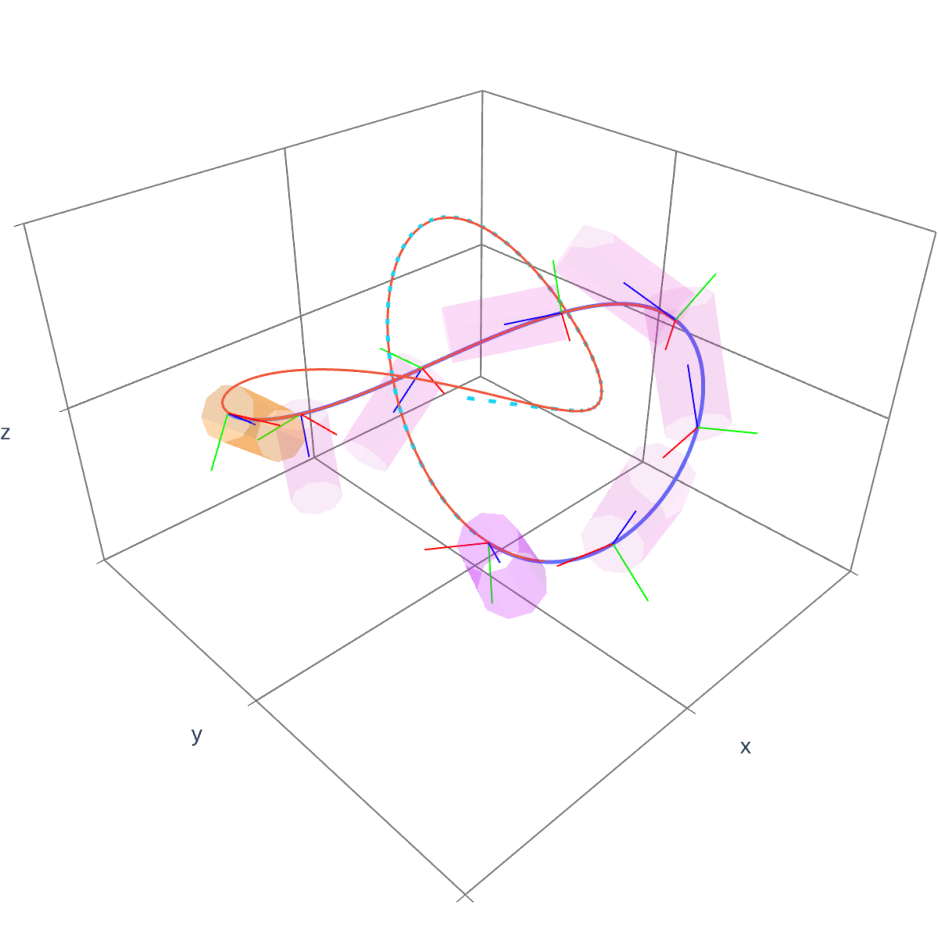
\includegraphics[width=0.32\textwidth]{../figures/adaptive_traj2.pdf}}
        \subfloat{\label{cc}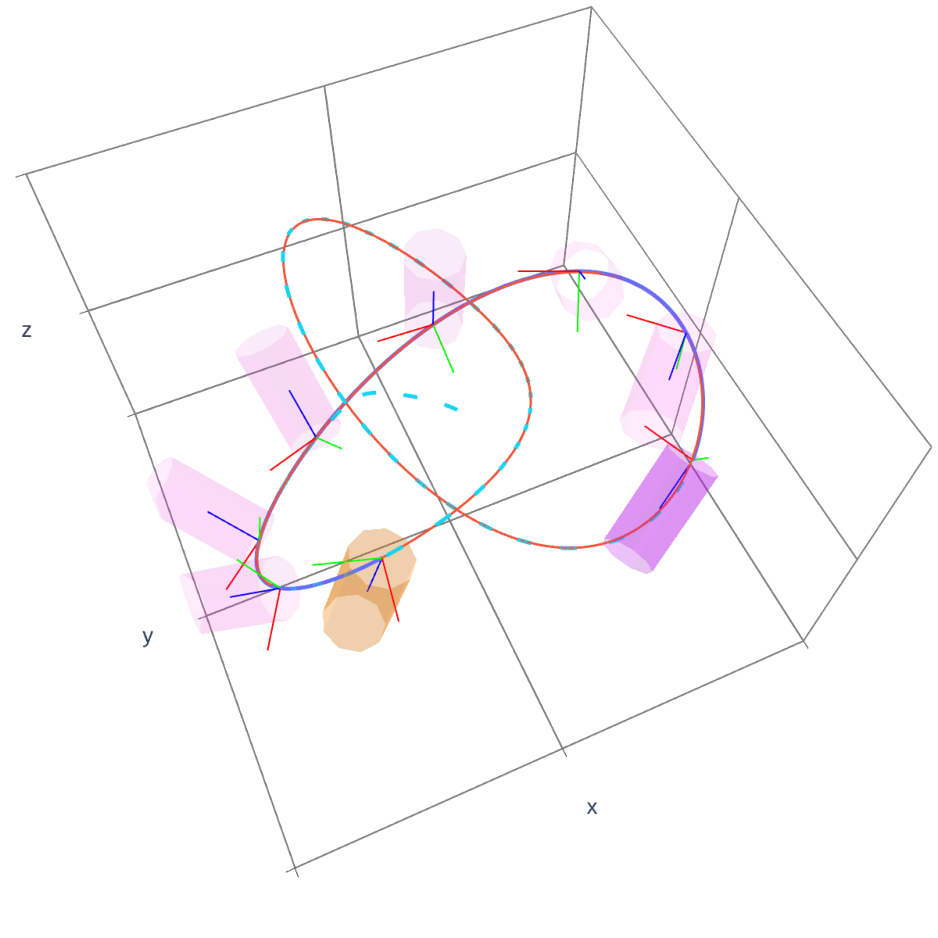
\includegraphics[width=0.32\textwidth]{../figures/adaptive_traj3.pdf}}
    \end{figure}
\end{frame}


\begin{frame}{Velocity error}
    \begin{figure}[ht!]
        \centering
        \def\svgwidth{.9\linewidth}
        {\scriptsize\import{../figures/}{adaptive_snorm.pdf_tex}}
    \end{figure}
\end{frame}

\begin{frame}{Distance}
    \begin{figure}[ht!]
        \centering
        \def\svgwidth{.9\linewidth}
        {\scriptsize\import{../figures/}{adaptive_distances.pdf_tex}}
    \end{figure}
\end{frame}
% !TeX root = Template Latex - Apresentacao - IFSP - SBV.tex
\section{Conclusion}
% \subsection{Conclusion and Future Works}

\begin{frame}

    \frametitle{Conclusion and Future Work}
    \begin{columns}[c]
        \begin{column}{0.6\linewidth}
            \begin{itemize}
                \item The vector field strategy is capable of driving systems in different Lie groups to track a desired curve;
                \item the work shows the possibility to use different distances in Euclidean space;
                \item the vector field can serve as a high-level controller, acting
                as a velocity reference for a lower-level dynamic controller.
            \end{itemize}
        \end{column}
        \begin{column}{0.4\linewidth}
            Future works include:
            \begin{itemize}
                \item Time-varying and self-intersecting curves;
                \item simpler distance functions;
                \item better optimization algorithms;
                \item nonholonomic constraints;
                \item validation in real systems.
            \end{itemize}
        \end{column}
        
    \end{columns}
\end{frame}

% \section{Referências}
% \begin{frame}[allowframebreaks]{Referências}
\begin{frame}{References}
\setbeamercolor{bibliography entry author}{fg=black}
\setbeamercolor{bibliography entry title}{fg=black} 
\setbeamercolor{bibliography entry location}{fg=black} 
\setbeamercolor{bibliography entry note}{fg=black}  
    % \setbeamercolor{bibliography item}{fg=black}
    % \setbeamercolor*{bibliography entry title}{fg=black}
    \setbeamerfont{bibliography item}{size=\footnotesize}
    \setbeamerfont{bibliography entry author}{size=\footnotesize}
    \setbeamerfont{bibliography entry title}{size=\footnotesize}
    \setbeamerfont{bibliography entry location}{size=\footnotesize}
    \setbeamerfont{bibliography entry note}{size=\footnotesize}
    \footnotesize\bibliography{IEEEabrv,referencias}
\end{frame}
% \begin{frame}

%     \frametitle{Conclusão e Trabalhos Futuros}

%     Slide n da conclusão...

% \end{frame}


% \begin{frame}
%     \begin{center}
%         \Huge{OBRIGADO!}
%     \end{center}
% \end{frame}


% exemplos de construções em LaTeX
% comente a linha abaixo para gerar a versão final
% \section{Exemplos}


\begin{frame}

    \frametitle{Título do Slide}

    Texto corrido normal .
    
    \begin{huge}
        Texto com fonte gigante.
    \end{huge}
    
    \begin{LARGE}
        Texto com fonte GRANDE.
    \end{LARGE}
        
    \begin{Large}
        Texto com fonte Grande.
    \end{Large}
    
    \begin{large}
        Texto com fonte grande.
    \end{large}
    
    \begin{normalsize}
        Texto com fonte normal.
    \end{normalsize}
        
    \begin{small}
        Texto com fonte pequena.
    \end{small}
        
    \begin{footnotesize}
        Texto com fonte do tamanho de nota de rosapé.
    \end{footnotesize}
    
    \begin{scriptsize}
        Texto com fonte do tamanho de letra manuscrita.
    \end{scriptsize}
        
    \begin{tiny}
        Texto com fonte minúscula.
    \end{tiny}        

\end{frame}


\begin{frame}

    \frametitle{Slide com Duas Colunas}
    
    \begin{columns}[t]
    
        \begin{column}{7cm}

            Conteúdo da coluna 1.

        \end{column}

        \begin{column}{7cm}

            Conteúdo da coluna 2.

        \end{column}

    \end{columns}
        
\end{frame}


\begin{frame}

    \frametitle{Slide com Blocos}
    
    Exemplos de blocos de texto. Cuidado para não abusar no uso, evitando que os slides fiquem muito ``carregados''.
    
    \begin{block}{Observação}
        Caixa de texto padrão.
    \end{block}
    
    \begin{exampleblock}{Exemplo}
        Caixa de texto de exemplo.
    \end{exampleblock}
        
    \begin{alertblock}{Importante}
        Caixa de texto de alerta.
    \end{alertblock}
    
    \definecolor{corFundoTitulo}{RGB}{95, 40, 113}
    \definecolor{corTextoTitulo}{RGB}{255, 255, 255}
    \definecolor{corFundoConteudo}{RGB}{114, 140, 166}
    \definecolor{corTextoConteudo}{RGB}{0, 0, 0}
    \begin{bloco}{Bloco com cores customizadas}{bg=corFundoConteudo,fg=corTextoConteudo}{bg=corFundoTitulo,fg=corTextoTitulo}
        Conteúdo
    \end{bloco}
         
\end{frame}


\begin{frame}

    \frametitle{Slide com Desenhos Usando Tikz}
    
    Desenhando formas...
    
    \begin{center}
        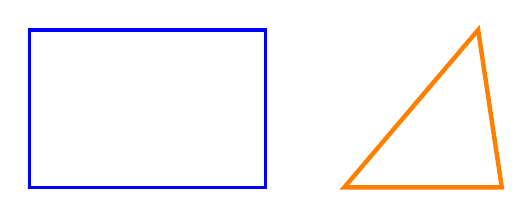
\begin{tikzpicture}[scale=1.0]
            \draw[blue, very thick] (0,0) rectangle (3,2);
            \draw[orange, ultra thick] (4,0) -- (6,0) -- (5.7,2) -- cycle;
        \end{tikzpicture}
    \end{center}
         
\end{frame}


\begin{frame}

    \frametitle{Slide com Desenhos Usando Tikz}
    
    Uma Máquina de Turing que realiza a operação subtração própria.
    
    \begin{center}
        \begin{tikzpicture} [scale=0.75, every node/.style={transform shape}, node distance = 3cm, on grid]

            \node (q0) [state,
                initial,
                initial text=Início
            ] {$q_0$};
            \node (q1) [state, right = of q0] {$q_1$};
            \node (q2) [state, right = of q1] {$q_2$};
            \node (q3) [state, right = of q2] {$q_3$};
            \node (q5) [state, below = of q0] {$q_5$};
            \node (q6) [state, below = of q1] {$q_6$};
            \node (q4) [state, below = of q2] {$q_4$};
                        
            \path [-stealth]
                (q0) edge node[above] {$0/B\rightarrow$} (q1)
                (q1) edge [loop below] node {$0/0\rightarrow$} ()
                (q1) edge node[above] {$1/1\rightarrow$} (q2)
                (q2) edge [loop below] node[right] {$1/1\rightarrow$} ()
                (q2) edge node[above] {$0/1\leftarrow$} (q3)
                
                (q3) edge [loop below] node {$
                    \begin{aligned}
                      0 &/ 0\leftarrow\\[-0.7ex]
                      1 &/ 1\leftarrow
                    \end{aligned}$} ()
                
                (q3) edge [bend right] node[above] {$B/B\rightarrow$} (q0)
                
                (q0) edge [bend right] node[left] {$1/B\rightarrow$} (q5)
                (q2) edge [bend right] node[left] {$B/B\leftarrow$} (q4)
                
                (q5) edge [loop below] node {$
                    \begin{aligned}
                      0 &/ B\rightarrow\\[-0.7ex]
                      1 &/ B\rightarrow
                    \end{aligned}$} ()
                                    
                (q5) edge node[above] {$B/B\rightarrow$} (q6)
                
                (q4) edge [loop below] node {$
                    \begin{aligned}
                      0 &/ 0\leftarrow\\[-0.7ex]
                      1 &/ B\leftarrow
                    \end{aligned}$} ()
                                    
                (q4) edge node[above] {$B/0\rightarrow$} (q6);
        
        \end{tikzpicture}
    \end{center}
         
\end{frame}


\begin{frame}

    \frametitle{Slide com Figura}
    
    \begin{figure}[!htbp]
       	\centering
       	\caption{Exemplo de figura (caption é opcional)}
       	\includegraphics[scale=0.3]{imagens/exemploFigura}
        \\\small{\textbf{Fonte:} Elaborada pelo autor (fonte é opcional)}%
     \end{figure}
         
\end{frame}


\begin{frame}

    \frametitle{Slide com Tabela}
    
    \begin{table}[!htbp]
       	\centering
       	\caption{Exemplo de tabela de 2 colunas (caption é opcional)}
       	\begin{tabular}{ c | c }
       		\hline
       		\textbf{Coluna 1} & \textbf{Coluna 2} \\ \hline
       		Dado 1a           & Dado 2a           \\ \hline
       		Dado 1b           & Dado 2b           \\ \hline
       		Dado 1c           & Dado 2c           \\ \hline
       		Dado 1d           & Dado 2d           \\ \hline
       	\end{tabular}
       	\\ \vspace{0.2cm}
       	\small{\textbf{Fonte:} Elaborada pelo autor (fonte é opcional)}%
     \end{table}
         
\end{frame}


\begin{frame}

    \frametitle{Slide com Quadro}
    
    \begin{quadro}[!htbp]
       	\centering
       	\caption{Exemplo de quadro (caption é opcional)}
       	\includegraphics[scale=.3]{imagens/exemploQuadro}
        \\ \vspace{0.2cm}
       	\small{\textbf{Fonte:} Elaborada pelo autor (fonte é opcional)}%
    \end{quadro}
         
\end{frame}


\begin{frame}

    \frametitle{Slide com Equação}
    
    \begin{equation}
        \sum_{i=1}^{n} i = \frac{n(n+1)}{2}
        \label{eq:exemplo}
    \end{equation}
         
\end{frame}


\begin{frame}

    \frametitle{Slide com Código Fonte}
    
    \centering
    \resizebox{10cm}{!}{%
        \lstinputlisting[language=Java]{fontes/ClasseExemplo.java} 
    }
    
\end{frame}


\begin{frame}

    \frametitle{Slide com Lista de Itens}
    
    \begin{itemize}
       	\item \textbf{Item 1:} texto...;
       	\item \textbf{Item 2:} texto...;
       	\begin{itemize}
       		\item \textbf{Subitem:} texto...;
       		\item \textbf{Subitem:} texto...;
       		\item \textbf{Subitem:} texto...;
       	\end{itemize}
       	\item \textbf{Item 3:} texto...;
       	\item \textbf{Item n:} texto....
    \end{itemize}
         
\end{frame}


\begin{frame}

    \frametitle{Slide com Lista Numerada}
    
    \begin{enumerate}
       	\item \textbf{Item:} texto...;
       	\item \textbf{Item:} texto...;
       	\begin{enumerate}
       		\item \textbf{Subitem:} texto...;
       		\item \textbf{Subitem:} texto...;
       		\item \textbf{Subitem:} texto...;
       	\end{enumerate}
       	\item \textbf{Item:} texto...;
       	\item \textbf{Item:} texto....
    \end{enumerate}
         
\end{frame}


\begin{frame}

    \frametitle{Formatação de Texto e Referências}
    
    Todas as macros que você utilizou na elaboração do seu documento podem ser usadas nas apresentações, com exceção do ambiente verbatim. Você poderá criar citações formatadas também, mas as referências não serão geradas em um slide, apenas serão exibidas no texto. Por exemplo:
    
    \begin{itemize}
        \item \cite{Abedi2014, Agaisse1995};
        \item \cite{AgapitoTenfen2014, BtNomenclature2016, Nelson2014};
        \item \citeauthorandyear{Agaisse1995};
        \item \citeauthorandyear{Abedi2014};
        \item \citeauthorandyear{BtNomenclature2016};
    \end{itemize}
         
\end{frame}

% % !TeX root = Template Latex - Apresentacao - IFSP - SBV.tex
% não mexa!

\begin{frame}<presentation:0>
    \addtocounter{framenumber}{-1}
    \bibliography{IEEEabrv,../references}
\end{frame}

\end{document}